\section{File usability and data access patterns}
One of the key parameters to assess how effective we are in using storage is to measure the access frequency after data placement. There are two extremes regarding data thermodynamics: a) cold data, where files are WORN (Write Once Read Never) and b) hot data, where files are expected to be accessed continuously and with high concurrency. But after studying data access patterns at several sites we observed that large fraction of our files are neither cold nor hot. The analysis objects files seems to lose popularity with time and the access rate decreases significantly after days/weeks, in (Fig. \ref{access}) it is shown the file access rates and file popularity on a Tier-1 and a Tier-2 as a function of time as a representative example.

\begin{figure}[h]
  \centering
  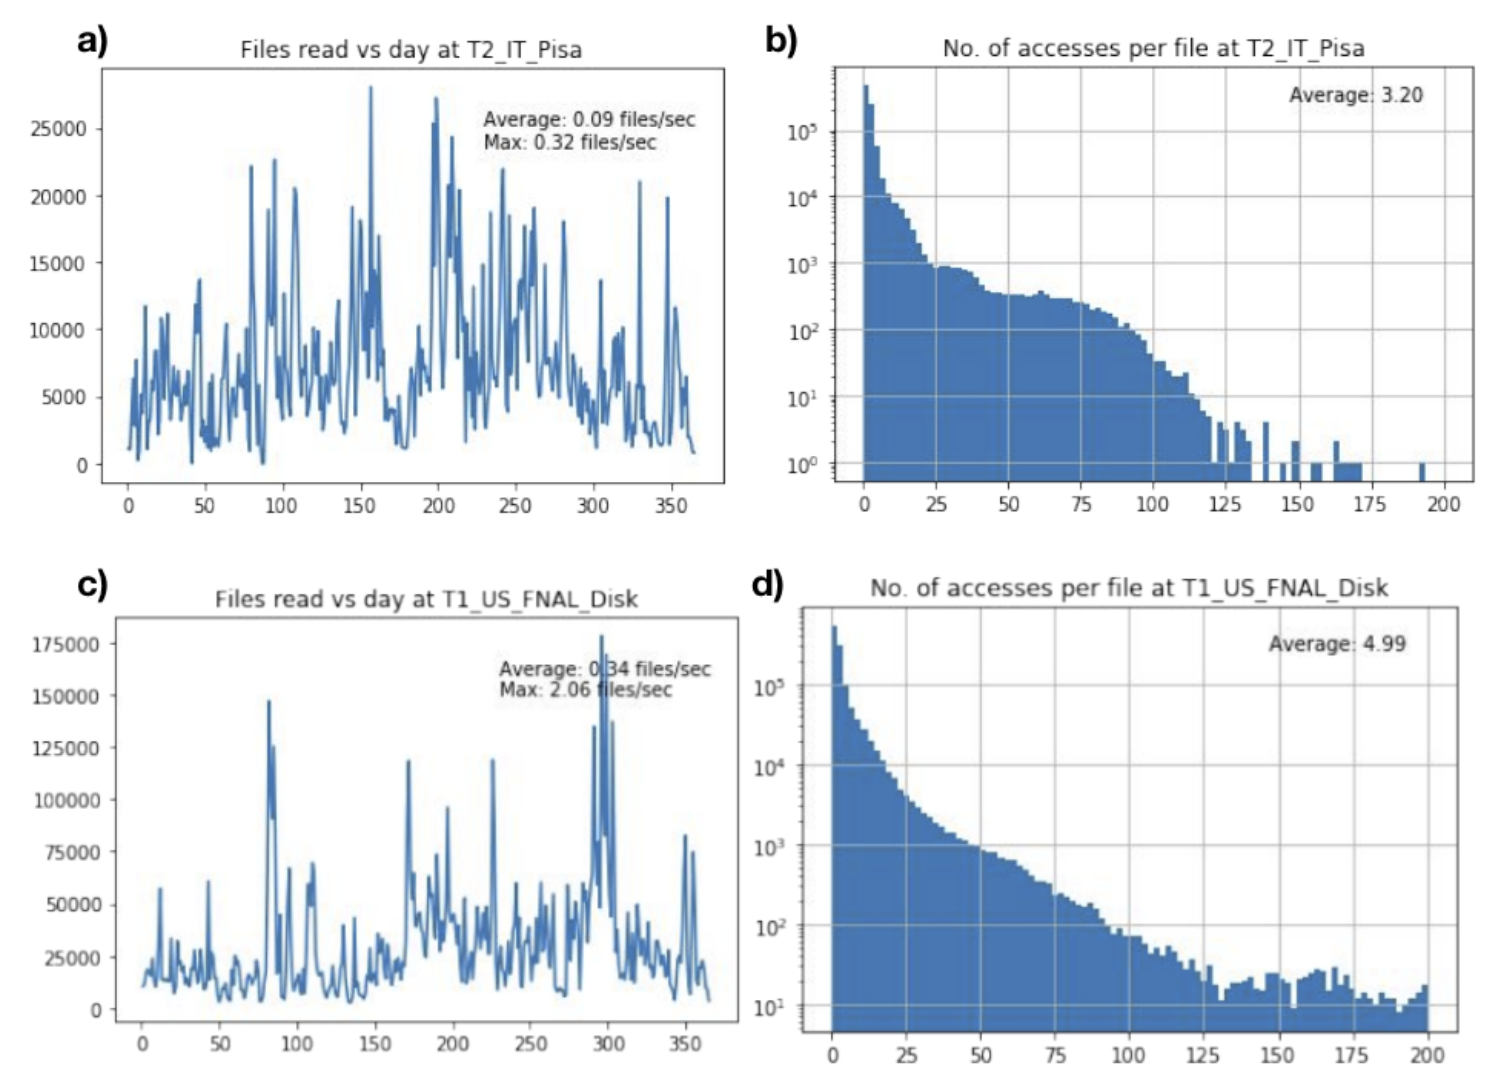
\includegraphics[height=8cm]{dataaccess-chep2019.png}
  \caption{{\em (left)} File popularity on a Tier-1 and a Tier-2 as a function of time (300 days). The plots above indicate that data is not accessed very often, it is most likely to be re-read within days after placement then the access drops substantially, almost two orders of magnitude.}
  \label{access}
\end{figure}

This provides an indication whether this type of data could be better handled with cache, so it is available when popular and gets superseeded with newer files once they are less demanded. In this way the space on disk at the computing sites is optimised for data being actively used, can this be completely delegate to a stateless cache? In parallel less frequently used data might be re-fetch again from the datalake (disk or tape) where the experiments will handle with the required Quality of Service (QoS) label to make use of the best cost/usage ratio.\\
We also observed a fundamental difference between Analysis and Production data. Analysis has higher re-use while production files have very few re-reads. The net effect is that running combined workflows on a site has the effect that production file push analysis data out of the storage/cache. This made us think that in the case we do not change much of the current infrastructure we would nevertheless benefit by changing the current model and favoring running predictable and time-defined workflows at the sites with less storage and favor less-predictable user analysis on sites with larger storage services.\\
Need to keep in mind these are preliminary studies based on a period of half a year. This need to be extended in further studies and also need to combine with staging and data deletion information. Nevertheless the results provide hints towards a cache-oriented storage.
